\subsection{Zadanie 3 -- Szukanie najliczniejszego zbioru wewnętrznie rozłącznych
	ścieżek}
\textbf{Treść: } Zaprojektuj algorytm, który dla zadanego grafu $G$
oraz wierzchołków $v, w \in V(G)$ znajdzie najliczniejszy
zbiór wewnętrznie rozłącznych wierzchołkowo ścieżek od 
$v$ do $w$ (innymi słowy, dla każdych dwóch ścieżek $P_1$ i $P_2$ z
tego zbioru jedynymi wspólnymi wierzchołkami $P_1$ i $P_2$ 
mogą być $v$ i $w$).

\textbf{Rozwiązanie: }
Graf wejściowy $G$ przekształcamy do grafu $G'$ w taki sposób, że
dla każdego wierzchołka $x \in V(G)$, tż. $x \not \in \{v, w\}$,
tworzymy wierzchołek $x'$, 
następnie przepinamy krawędzie wyjściowe z $x$ do $x'$ oraz 
dodajemy krawędź $xx'$. Rysunek \ref{fig:zad43_fig} wizualizuje
wyżej opisany zabieg.

\begin{figure}[H]
	\centering
	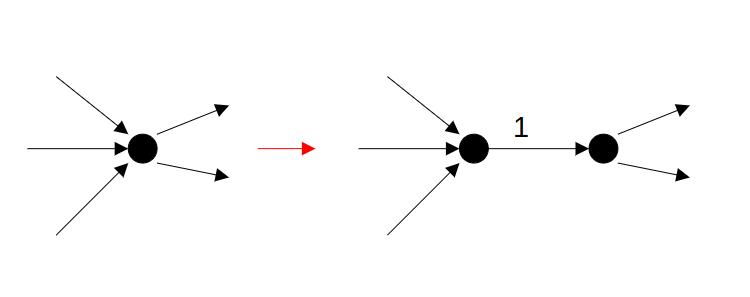
\includegraphics[width=0.4\textwidth]{data/zad43.png}
	\caption{  }
	\label{fig:zad43_fig}
\end{figure}

Wywołujemy Forda-Fulkersona na grafie $G'$, który zwróci nam 
wartość maksymalnego przepływu oraz przepływ $f$. Aby zapisać ścieżki
tworzymy graf $G''$, w którym usuwamy wszystkie krawędzie $e \in E(G)$,
tż., $f(e) = 0$. Dla każdego sąsiada $v$ idziemy do $w$, odkładając
napotkane wierzchołki do na listę. Zwracamy wszystkie listy. 

\subsection{Zadanie 4 -- Znajdowanie najmniejszego przekroju w sieci}
\textbf{Treść: } Przekrojem sieci $(G, c, s, t)$ 
nazywamy podział zbioru $V(G)$ na 
rozłączne zbiory $S$ i $T$ taki, że $s \in S$
oraz $t \in T$. Przepustowość takiego przekroju to suma
$\sum_{v\in S,w\in T} c(vw)$.
Zaprojektuj algorytm, który znajdzie przekrój 
o najmniejszej przepustowości w danej sieci przepływowej.

\textbf{Rozwiązanie: }
Rozwiązanie polega na uruchomieniu algorytmu Floyda-Fulkersona, a
następnie przebadaniu sieci rezydualnej $R$ dla maksymalnego przepływu $f$
zwróconego przez ten algorytm.

Uruchamiamy DFS lub BFS w celu znalezienia wszystkich osiągalnych wierzchołków 
z $s$ w sieci rezydualnej $R$. Zbiór osiągalnych wierzchołków $S$ oraz 
$\overline{S} = V(G) \setminus S$ stanowią podział o najmniejszej 
przepustowości.

\subsection{Zadanie 5 -- Algorytm Dinica}
\textbf{Treść: } Niech $R$ będzie siecią rezydualną 
dla pewnej sieci przeplywowej $(G, c, s, t)$ i przepływu $f$; 
niech $d$ będzie
odległością (w sensie liczby krawędzi) od $s$ do $t$ w $R$. 
Przez przeplyw blokujący w $R$ rozumiemy przepływ $f'$ w R taki,
że każda ścieżka od $s$ do $t$ w $f'$ ma dokładnie 
$d$ krawędzi oraz dla każdej ścieżki o $d$ krawędziach od $s$ do $t$ w $R$,
przynajmniej jedna krawędź tej ścieżki jest nasycona przez $f'$.
\begin{itemize}
	\item[a)] Zaprojektuj algorytm, który znajdzie przepływ blokujący w czasie $O(nm)$
	\item[b)] Skonstruuj algorytm rozwiązujący problem maksymalnego przepływu w czasie $O(n^2m)$
\end{itemize}
\textbf{Rozwiązanie: }

\begin{defi}
	Niech $R$ będzie siecią rezydualną dla pewnej sieci przepływowej
	$(G, c, s, t)$ oraz przepływu $f$. Niech $d$ będzie odległością w sensie
	liczby krawędzi od $s$ do $t$ w $R$.
	
	Przez przepływ blokujący w $R$ rozumiemy przepływ $b$ w sieci
	$(R, c_f, s, t)$, taki, że każda ścieżka od $s$ do $t$ 
	w $b$ ma dokładnie $d$ krawędzi oraz dla każdej ścieżki o $d$ 
	krawędziach od $s$ do $t$ w $R$, przynajmniej jedna krawędź tej ścieżki
	jest nasycona przez $b$.
\end{defi}

BFS + usuwanie niepotrzebnych krawędzi w $R$ w celu utworzenia tzw. 
grafu warstwowego, potem DFS w celu przejscia po kazdej ścieżce
i utworzenia przepływów.

\textbf{Rozwiązanie b: }

\begin{algorithm}[H]
	\caption{Algorytm Dinica}
	\begin{algorithmic}[1]
		\Procedure{Dinic}{($G, w, s, t$): sieć}
		\State Niech $f$ to zerowy przepływ w sieci $(G,c,s,t)$
		\State Utwórz sieć rezydualną $(R, c_f)$ dla wejściowej 
		sieci przepływowej oraz dla $f$ 
		\While{Istnieje ścieżka powiększająca w $R$}
		\State Znajdź przepływ blokujący $f'$ w sieci ($R, c_f$, $s$, $t$)
		\State Powiększ $f$ o $f'$
		\State Uaktualnij $(R, c_f)$
		\EndWhile
		\State \Return $f$
		\EndProcedure
	\end{algorithmic}
	\label{alg:dinic}
\end{algorithm}

\subsection{Zadanie 6 -- Wyznaczanie pesymistycznej wydajności w sieci}
\textbf{Treść: } Przypuśćmy, że mamy daną sieć przewodową składającą 
się z $n$ węzłów (w tym jeden serwer) i $m$
połączeń między węzłami, przy czym każde połączenie ma pewną 
przepustowość wyrażoną w kB/s. Zakładamy, że
każdy węzeł może jedynie odbierać dane i przesyłać je 
dalej (w szczególności, zabronione są modyfikacje danych przed
ich przesłaniem). Przez pesymistyczną wydajność sieci 
rozumiemy najwiekszą wartość $w$ taką, że serwer jest w stanie
wysyłać jednocześnie do każdego innego węzła dane w ilości $w$ kB/s.

Zaprojektuj algorytm, który wyznaczy pesymistyczną wydajność zadanej sieci.

\textbf{Rozwiązanie: }
Rozwiązanie polega na połączeniu wszystkich routerów z ujściem $t$ krawędziami 
o przepustowości 1. Jeżeli po wywołaniu algorytmu znajdującego maksymalny
przepływ każda z krawędzi do ujścia $t$ jest nasycona, to 
zwiększamy przepustowość każdej z tych krawędzi o 1 i ponawiamy próbę.
Ostatnia liczba dla której wszysktkie krawędzie były nasycone to 
szukane $w$.


Powyższe rozumowanie można zoptymalizować korzystając z 
binarnego przeszukiwania. Jako maksimum przyjmujemy
sumę przepustowości na krawędziach
wychodzących z $s$ 
(bo $\text{val} f_{max}$ jest nie większe niż
wartość dowolnego przekroju), a jako minimum -- 1.

\begin{algorithm}[H]
	\caption{Wyznaczanie pesymistycznej wydajności}
	\begin{algorithmic}[1]
		\Procedure{FindPesimisticEfficiency}{($G, c, s, t$): sieć}
		\State $V' \gets V(G) + \{t\}$
		\State $E' \gets E(G) + \{vt : v \in V' \setminus \{s, t\} \}$
		\State $G' \gets (V', E')$
		\State $R \gets \sum_{v \in N(s)}c(sv)$
		\State $L \gets 1$
		\While{$L < R$}
		\State $w = \lfloor \frac{L + R}{2} \rfloor$
		\For{$e \in E'$}
		\State $c(e) \gets w$
		\EndFor 
		\State $f \gets$ Ford-Fulkerson($G'$, $c$, $s$, $t$)
		\If{$\forall_{e \in E'} f(e) = w$}
		\State $L \gets w + 1$
		\Else
		\State $R \gets w - 1$
		\EndIf
		\EndWhile
		\State \Return $w$
		\EndProcedure
	\end{algorithmic}
	\label{zad46}
\end{algorithm}

\subsection{Zadanie 8}
\textbf{Treść:} Rozważmy pociąg, który zatrzymuje się na stacjach 
numerowanych liczbami od 1 do $n$. Pociag może
przewozić jednocześnie P pasażerów. Dla każdej pary stacji 
$i$, $j$, gdzie $i < j$, mamy daną liczbę $b_{ij}$ pasażerów chcących
przejechać od stacji $i$ do $j$ oraz koszt jednego takiego biletu $c_ij$ .
Zaprojektuj algorytm, który określi, komu należy sprzedać bilety tak, 
aby zmaksymalizować zysk (tzn. sumę kosztów
sprzedanych biletów).